\iffalse \bibliography{include/backmatter/magnus,include/backmatter/philip} \fi
\chapter{Introduction}
%funneling from the world to the actual problem 
In order for organisations to remain competitive, there is a need to continuously improve time to market for new features and services. The societal transformation of moving from a product economy to a service economy has affected the way organisations deliver software \cite{mckinsey}. Products are required to move from business requirements to delivery as fast as possible. This societal transformation from a product to service economy has given rise to a number of tools and methodologies to bring more value to customers in a shorter amount of time. Continuous integration (CI) and continuous deployment (CD) are software engineering concepts that have become strongly adopted by organisations in order to deal with the need for more agility. More agility is required in order to rapidly respond to change in customer requirements in a market that is constantly evolving. With a well designed CI and CD process, organisations can deliver new features to customers in a short amount of time and on a regular basis. The popularity and success of CI and CD is strongly based on pure software products. However, other disciplines within software engineering are attracted to the benefits CD offers. Such applications are within the domain of internet of things and cyber-physical systems (CPS), as identified in \cite{gonz,cberger,2iot}, where the continuous deployment of features is becoming an important factor.\\

Cyber-physical systems are computer systems collaborating and coordinating to control physical resources that interact with their surroundings \cite{cps}. CPS's are becoming an integral part of society and are already available to consumers in modern vehicles. Collision avoidance, autonomous parking and autonomous highway driving are some examples of CPS's within the automotive domain. By nature, such systems are very complex in their design and development, involving multiple software and hardware components of different types and architectures. The cyber-physical systems discipline has emerged as a direct response to deal with such complexity, requiring expertise from three major disciplines: (1) communication in heterogeneous networks, (2) embedded and real-time systems and (3) control systems \cite{gonz}. \\

The continuous deployment of features in a CPS is challenging due to a number of reasons. Namely, the system is typically resource constrained so scaling up hardware is limited. Furthermore, a CPS requires real-time operations so any additional overhead to performance should be taken with care. Additional overhead can introduce latency that may impact an applications timing requirements which could result in a catastrophic effect. CPS's typically interact with their surroundings so safety is of a high concern. \\

Deploying any complex system to a production environment is a challenging procedure. Using virtual machines simplifies the deployment process by packaging the application in a isolated sand-boxed environment. Shipping an application pre-installed in a virtual machine has some serious benefits. However, as real-time requirements are crucial to CPS's, the cost to performance must be identified if considering virtualization as a deployment platform.\\

Virtualization can be done with a fully fledge virtual machine (e.g Oracle VirtualBox) or by using lightweight virtual containers. Virtual machines bring higher overhead as they require full copy of a operating system as well as virtualising hardware \cite{7093032}, so they are not suitable for vehicular CPS's. A more lightweight approach is to use virtual containers that share the host operating system (OS) rather than encapsulating an entire OS stack. Containerizing an application brings additional benefits. Runtime orchestration can be better controlled when executing applications that are sand-boxed from each-other where resources can be controlled and limited. A/B testing can also be performed between different containers, but above all, containers deliver an application in a highly portable environment.\\

This study aims to uncover the performance impact of using virtual containers for software deployment in the context of autonomous vehicles. Self driving vehicles require minimal delays during runtime to allow real-time computations to enable autonomous driving that is safe. Minimal time-delay is a fundamental concern for allowing lane-following, decision making, and other computations utilized by the autonomous vehicle to interact with its surroundings. The software composed for self-driving vehicles can benefit by the use of virtualization, during development (such as safe roll back and independent versioning) as well as post-development to ship updates and patches. In order to consider the use of virtual containers for CPS's, one needs to first understand the overhead that is introduced to ensure that the system meets the real-time requirements for safe driving.\\

Methods of experimentation are used to uncover the scheduling precision and input/output performance of two sample applications realised with the open source development architecture for CPS's, OpenDaVINCI \cite{OpenDaVINCI}. Runtime latency of containerising two sample applications is mitigated by using a real-time enable Linux kernel and comparing it to a vanilla Linux kernel. The Docker containet manager is the chosen techonology for containerising the applications due to being open source and highly successfull since its release in 2008 \cite{docker}. Furthermore, the results of the study are replicated and validated by running the experiment on a self-driving vehicle that participated in the 2016 Grand Cooperative Driving Challenge in The Netherlands.

%Software deployment for CPS is difficult as there are many aspects to put into consideration. Typically,  CPS are resource constrained, meaning that you cannot scale up hardware exponentially as you typically do not have the physical space for it. Secondly, real-time requirements are needed, so any SD tools needs to be lightweight. Finally, there are safety concerns since CPS typically interact with their surroundings. 

%---------------------------------------------------%
\section{Background}
This section introduces the technologies and concepts related to this paper.
%latency mitigated by modifying operating sytem to provide more determinism 
%linux foundation announced fully support rt linux 
%virtualization can be done with fully-fledged Virtual Machines or lightweight containers. VMs  incure higher ovhead but better protection and so are not suitable for autonomous vehicles.  Therefore we adopt containers and strive to minimize latency by real-time Linux kernel
%containers very efficiently share and utilize CPU and memory resources, 

\subsection{Cyber Physical Systems}
%Software deployment for CPS is difficult as there are many aspects to put into consideration. Typically,  CPS are resource constrained, meaning that you cannot scale up hardware exponentially as you typically do not have the physical space for it. Secondly, real-time requirements are needed, so any SD tools needs to be lightweight. Finally, there are safety concerns since CPS typically interact with their surroundings. 

%compact middleware OpenDaVINCI written in standard C++, can be used on a variety of POSIX OS. we use ODV to have a lean, portable and high-performance hardware and OS abstraction layer for typical programming idioms like concurrency, data storage and communication

Comparing a real-time system with an ordinary application, the difference is seen in how the execution of code is made. For an ordinary application an algorithm is executed once to provide a result output from an input without any specific time constraints. However, a real-time system is recognised by its time constrain characteristic as the system is configured to execute an algorithm within a specified time-slice, i.e. \texttt{10milliseconds}.\\

Systems used for autonomous self-driving vehicles utilises a number of different algorithms to enable the self-driving functionality. The responsibilities for these algorithms is presented in figure \ref{containers}, where different responsibilities are broken down. One algorithm is responsible for processing the camera feed, another algorithm is responsible for detecting lanes within the captured images from the camera, and another is responsible for make a decision to steer, break, or accelerate the vehicle depending on the content of the feed. All these algorithms are embedded in a middle-ware application which sets the time constraints of the algorithms and handle the interface between the different nodes. This research looks to utilise an open source middle-ware named OpenDaVINCI. OpenDaVINCI is an application specifically developed for autonomous self-driving vehicles which is implemented in several research projects \cite{OpenDaVINCI}.


\subsection{Software Deployment}
Software deployment is a crucial part of the software development, it refers to the activities which makes the software system available for use \cite{carzaniga1998characterization}. The process contains a number of activities which all play into the life cycle of a software system with the goal to implement into the runtime environment where the system is set to operate live. These activities are namely: \\

\textbf{Release} – is the activity of packaging the software for delivering it to the end user. This includes processes such as including the software's requirements and dependencies to external components, such as libraries and applications. It also includes the process of advertising – the process of informing interested parties about the software being released.\\
\textbf{Install} – refers to the activities of assembling all required resources for the runtime environment. It consists of two specific process, namely \textit{transfer} and \textit{configuration}. Where the former is the process of transferring the software from the developer to the runtime environment and the later is the process of making the software ready for activation.\\
\textbf{Activate} – is the process of executing the software and all dependent applications in the runtime environment.\\
\textbf{Deactivate} – is the opposite of the \textit{activate} activity.\\
\textbf{Update} – is the activity of updating the version of the running software which consists of similar activities of the \textit{install} activity.\\
\textbf{Adapt} – refers to the process of ensuring that the updated version is running correctly in the runtime environment.\\
\textbf{Deinstall} – is the activity of decommissioning the running software and includes sub-activities such as removing the external libraries and components.\\
\textbf{Derelease} – is the final activity which includes the process of advertising the withdrawal of the software system.\\

All these activities differ in how they are executed depending on the software engineering paradigm utilised for the software project. In traditional software engineering practices, e.g. the waterfall model, seeks to execute the software deployment process at the end of the software's development cycle. Whereas more novel software engineering practices aim to execute the software deployment process continuously throughout the software's development cycle. In state-of-art software engineering practices such as continuous integration and continuous deployment, requires software to be deployed daily \cite{meyer2014continuous}. Such requirements can easily make the process of software deployment exhausting and complex, where software tools such as Docker would simplify these processes greatly. Docker simplifies processes found within each of the software deployment activities, as it provides the runtime environment before the software deployment process has begun. The development environment is a clone of the production environment thus transferring the deployment processes from the live production server to a confined a secure location where the deployment process does not affect the usability of the current running software.\\


\begin{figure}[ht]
\centering
     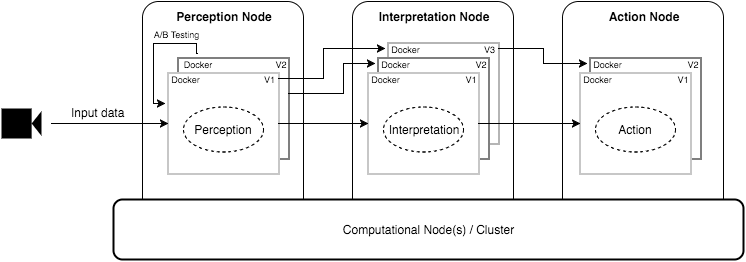
\includegraphics[width=1.0\textwidth]{./figure/containers.png}
      \caption{Run-time environment using Docker.}
       \label{containers}
\end{figure}

Figure \ref{containers} displays a deployment strategy design utilising Docker in the context of self-driving vehicles. The responsibilities are broken down into three computational nodes in which Docker containers are running instances of the code base independently. Each Docker container can run different versions of the separate nodes, where the interpretation node has three versions running separately. Version one (denoted V1) in each node represents the latest working configuration while other versions are run to test code which is still under development. Aforementioned, this allows for safe and simple roll-backs in the event of buggy code or degraded performance. Furthermore, multiple versioning of the same Docker container allows for split testing between different containers to take place. With an always functioning configuration, the development team can demonstrate the current status to stakeholders at any point in the development cycle. The ability to demonstrate the product at any point in the development phase adds to the business value as possible investors or stakeholders can see a functioning product even though it is currently under development. With current approaches this is possible, however it is not as straightforward and easily implemented as in cases which utilizes Docker for its deployment strategy.

\subsection{Container-Based Virtualization}
%process isolation and application portability

Docker is an open source light-weight container environment which was initially launched in 2013 and has gained ground rapidly with its simplicity. The environment offered by Docker simplifies the process of software deployment by packaging all dependencies into a light-weight virtualisation container which ensures that all instances of the software is utilising the same dependent libraries. The functionality provided by Docker is comparable with virtual machines as both are virtualised environments where software applications can be executed with all dependent libraries and applications are installed. However, Docker, in contrast to virtual machines, is a light-weight alternative as it communicates directly to the host machine's kernel. A virtual machine has the additional level of a virtual operating system which adds complexity which does not directly speak with the host machine's kernel. With the benefit of packaging the dependent libraries and applications into the container, software developers can avoid uncertain deployments where library versions may differ between the developers' development environments and the live production environment. Docker presents further benefits such as safe roll-back between different software versions which provides projects' the ability to always be able to fall back on application versions which are known to function correctly. By providing these benefits project managers can feel secure in that there always exists a working runtime environment in the scenario of a new failing deployment.\\

The container in which Docker packages all dependent libraries and applications are referred to as a Docker image. This image contains everything which is required for an application to be executed. In the case of self-driving vehicles such dependencies may be image processing libraries such as OpenCV and the middle ware which enables the real-time application. When executing an application within Docker, a container is executed with based on the Docker image which consists of the installed libraries. This software design allows for split testing of software as the same application can be executed multiple times without clashing with the other contained application. Thus being optimal for testing different versions of the same application simultaneously while knowing there is no interference between the executed applications.

\subsection{Task Scheduling} %kernel and cpu scheduler
An operating system handles the communication between the software and the hardware, more specifically the operating system kernel acts as the interface between hardware and software. As an operating system is running a vast amount of processes simultaneously there is a need to prioritise and select which processes to run at what time. Each process utilises the CPU to make the computations required for the process to operate. The CPU is a powerful piece of hardware which can handle the same number of processes as it has cores and threads, i.e. an general Intel Core i7 processor has 4 cores and two threads per core amounting to 8 total processes simultaneously. However an operating system may run more processes than the CPU can process simultaneously. To manage this flood of processes a software component referred to as the \textit{CPU scheduler} which is configured by the kernel and is implemented to ensure that there is a queuing system set up for all processes running on the system. The \textit{CPU scheduler} acts as a traffic police in a busy intersection, handling a queue of all the processes running on the system by prioritising some processes ahead of other processes. The \textit{CPU scheduler} may act and prioritise differently depending on what rules have been set for it to follow.\\

The Linux OS CPU scheduler implements a FIFO (first-in-first-out) approach with two process scheduler algorithms, namely a time-sharing algorithm and a real-time algorithm. Where the former is a \textit{fair} scheduler algorithm trying to distribute the system's CPU resources equally over all processes in the queue ensuring that no process is completely starved. The later is an algorithm which prioritises the processes based on their set importance, where a higher prioritised process is provided more resources in comparison with a lower process. However, the generic Linux kernel version does not allow for any resource cut-off for processes utilising the CPU. A higher prioritised process will therefore not be able to utilise 100\% of the CPU's resources if there are other processes already using the CPU. This is not remarkable for a general purpose operating system running non-time sensitive applications. For a RT system it is crucial to ensure that the highest level process can interrupt any running processes at any point in time. An RT\_preempt kernel may be implemented to cope with such a design. This kernel design allows the scheduler to preempt any running process of lower priority than the requested process. Furthermore, the RT\_preempt kernel locks any resource utilised by a RT prioritised process.

\subsection{Real Time System and Scheduling Precision}
To understand the performance impact of utilizing Docker containers for the deployment strategy, the experiments of this research will analyse the scheduling precision of the automotive real-time application. The application executes computations within elements referred to as time-slices. The time-slice is a specification of time allocated for the algorithm to execute and deliver a result. A real-time application running at \texttt{100hertz} executes 100 time-slices per second, which results in one time-slice being \texttt{10milliseconds} or \texttt{0.01second}. The \texttt{10milliseconds} time-slice is the time deadline set for the specific application, which is the maximum time allowed for the assigned algorithm to finish its computations. In scenarios where the algorithm utilizes less than the assigned time-slice the application will sleep for the remaining time until it fires a new execution. Assuring that the application sleeps for the specified time is a responsibility assigned to the operating system scheduler. Where the scheduler initiates processes which are sleeping and wishes to fire a new time-slice. Other than the assigned algorithm, the real-time application consists of code which is responsible for controlling the sleep of the time-slices. Therefore a part of the time-slice has to be consumed to execute the required code. The time consumed by the code which controls the sleep of the application is referred to as the middle-ware overhead which is part of what is used for measuring the scheduling precision of the execution environment.\\

Scheduling precision refers to how accurately the application executes the specified algorithm from the point of firing the time-slice until the algorithm begins its computation. Further accuracy is measured between the point of where the algorithm finishes its computations until the real-time application sleeps. Lastly, measurements are done to see whether the \texttt{sleep} function of the system actually sleeps for the remainder of the time-slice or if it overstays the specified time deadline.\\

The limitations of each execution environment can be identified by understanding how much time each part of the required code occupies the time-slice. The less time required for executing the code outside of the assigned algorithm the more deterministic a system is said to be. In a scenario where the assigned algorithm requires 80\% of the time-slice to execute the code, it is assumed that the application will sleep for the remaining 20\%. However, as there exists additional operations surrounding the algorithm the application might sleep 18\% whereas 2\% is required for the surrounding code to execute. If the application still sleeps 20\%, executes the algorithm for 80\%, and uses 2\% for the required code it will overstay its time-slice by 2\% thus rendering the application less deterministic. It is the time available for the algorithm the experiments will seek to identify to inform software engineers of how much of the time-slice can be used for effective computations, i.e. time available for generating a result.


%---------------------------------------------------%



%---------------------------------------------------%
\section{Problem Domain \& Motivation}
% This is a dedicated section for problem and motivation, you should not deviate too much from our domain and context
%---------------------------------------------------%



%---------------------------------------------------%
\section{Research Goal \& Research Questions}
% We need rationales to explain what we expect from these RQs. Further, it would be nice to have some preparation sentences that would justify asking these questions and not others
%---------------------------------------------------%



%---------------------------------------------------%
\section{Contributions}
% The contribution made to the research community by answering the RQs.} 
% Many studies have analyzed virtual machines and containers to compare their performance cite. 

While this research bases its merits on a narrow field of interest, its application can be used for a broad audience within the research community as well as for organisations interested in adopting new technology to improve software deployment for real-time systems. As more segments of today’s society are becoming automated and reliant on software decision making, real-time systems plays an integral part of this development. Financial, aviation, and vehicle systems are just a few examples of domains with systems that are highly sensitive to time delays. A self-driving vehicle has to interpret its surroundings in real-time where any delay can have a catastrophic effect. Similarly, applications in the financial domain have to react to market fluctuations within nanoseconds to avoid loss on investment.

\section{Scope}
% In this section we will introduce the scope which is self-driving vehicles. The hardware we are using is in-line with actual hardware used in autonomous vehicles. The software development architecture used for our experimental units have been adopted in research projects involving the actual development of autonomous vehicles. We do not aim for our results to be valid in other types of autonomous systems, such as drones.

\section{Structure of the thesis}
% Summary: In this section we will introduce a typical outline of the paper.}
%---------------------------------------------------%